\documentclass[12pt]{article}
\usepackage{geometry}
\geometry{a4paper}


\usepackage{color}
\usepackage{hyperref}
\usepackage{amsmath}
\usepackage{amsfonts}
\usepackage{amssymb}
\usepackage{graphicx}
\usepackage{tcolorbox}
\usepackage{listings}
\usepackage{here}
\usepackage{txfonts}
\usepackage{algorithm}
\usepackage{algorithmic}
\usepackage{siunitx}
\usepackage{xcolor}
\usepackage{ascmac}
%\usepackage{fancybx}

\lstset {language = c++,
  basicstyle = \ttfamily \scriptsize,
  commentstyle = \textit,
  frame = tRBl,
  framesep = 5pt,
  showstringspaces = false,
  numbers = left,
  stepnumber = 1,
  numberstyle = \tiny,
  tabsize = 2,
  keywordstyle = \bfseries \color{blue},
  stringstyle=\color{magenta},
  commentstyle=\color{red},
  morecomment=[l][\color{red}]{\#}
  showstringspaces=false, % don't mark spaces in strings
}
\newcommand{\bi}[1]{\mathbf{#1}}
\newcommand{\bs}[1]{\boldsymbol{#1}}  % bold for greek characters
\newcommand{\bbR}{\mathbb{R}}

\author{Nobuyuki Umetani}

\title{LU Decomposition \footnote{This is a memorandum to write down what the forgetful author studied a long time ago. Surely it contains many mistakes. Excuse me. It is appreciated if you let me know if you have any comments or suggestions. }}

\begin{document}
\maketitle
\tableofcontents

\section{Introduction}

We often use LU decomposition, which is a kind of direct method to solve a matrix. LU factorization is a method of expressing a coefficient matrix by the product of a lower triangular matrix and an upper triangular matrix. By using the fact that it is a triangular matrix after the LU factorization, simultaneous linear equations can be solved at high speed using forward / backward substitution. Here we briefly describe the method of LU decomposition. In explaining the LU factorization, the block LU decomposition will be explained first. LU factorization is obtained by repeating the special case of block LU decomposition many times.

\section{Block decomposition}


\subsection{Block LU decomposition}

Consider the following square matrix
%
\begin{eqnarray}
\left[\begin{array}{ll}
\bi{A} & \bi{B}\\
\bi{C} & \bi{E}
\end{array}\right],
\end{eqnarray}
%
where $\bi{A}$,$\bi{B}$,$\bi{C}$ and $\bi{E}$ are also matrices (we use $\bi{E}$ instead of $\bi{D}$ here to avoid confusion with a diagonal matrix).
%
It is easy to check that this matrix can be written as the multiplication of two matrices
%
\begin{eqnarray}
\left[\begin{array}{ll}
\bi{A} & \bi{B}\\
\bi{C} & \bi{E}
\end{array}\right]
=
\left[\begin{array}{ll}
\bi{I} & 0\\
\bi{C}\bi{A}^{-1} & \bi{I}
\end{array}\right]
\left[\begin{array}{ll}
\bi{A} & \bi{B}\\
0 & \bi{E} - \bi{C}\bi{A}^{-1}\bi{B}
\end{array}\right].
\end{eqnarray}
%
The decomposition results in a block lower triangle matrix and a block upper triangle matrix.
%
Thus, this decomposition is called block LU decomposition.
%
To be more precise, there are several types of block LU decomposition and this decomposition is a special case where a diagonal block of the lower block triangle matrix becomes a unit matrix.
%
The lower right entry of  the right matrix is called \emph{Shur complement} and sometimes write $\bi{S}$.
%
\begin{equation}
\bi{E} - \bi{C}\bi{A}^{-1}\bi{B} = \bi{S}
\end{equation}
%


\subsubsection{Inverse matrix of block lower triangular matrix}

You can easily check the following equation by hand:
\begin{eqnarray}
\left[\begin{array}{ll}
\bi{I} & 0
\\ \bi{C}\bi{A}^{-1} & I
\end{array}\right]
\left[\begin{array}{ll}
\bi{I} & 0\\
-\bi{C}\bi{A}^{-1} & \bi{I}
\end{array}\right]
=
\left[\begin{array}{ll}
\bi{I} & 0\\
0 & \bi{I}
\end{array}\right]
\end{eqnarray}
%
This mean that the inverse of the block lower triangle matrix is:
%
\begin{eqnarray}
\left[\begin{array}{ll}
\bi{I} & 0\\
\bi{C}\bi{A}^{-1} & I
\end{array}\right]^{-1}
=
\left[\begin{array}{ll}
\bi{I} & 0\\
-\bi{C}\bi{A}^{-1} & \bi{I}
\end{array}\right]
\end{eqnarray}




\subsubsection{Solving a linear system using the block LU decomposition}

Consider the following linear system.
%
\begin{eqnarray}
\left[\begin{array}{ll}
\bi{A} & \bi{B}\\
\bi{C} & \bi{E}
\end{array}\right]
\left\{\begin{array}{l}
\bi{x}_A\\
\bi{x}_B
\end{array}\right\}
=
\left\{\begin{array}{l}
\bi{y}_A\\
\bi{y}_B
\end{array}\right\}
\end{eqnarray}


Let use have the block LU decomposition on the coefficient matrix. 
%
\begin{eqnarray}
\left[\begin{array}{ll}
\bi{I} & 0\\
\bi{C}\bi{A}^{-1} & I
\end{array}\right]
\left[\begin{array}{ll}
\bi{A} & \bi{B}\\
0 & \bi{S}
\end{array}\right]
\left\{\begin{array}{l}
\bi{x}_A\\ \bi{x}_B
\end{array}\right\}
=
\left\{\begin{array}{l}
\bi{y}_A\\
\bi{y}_B
\end{array}\right\}
\end{eqnarray}
where  I wrote Shur Complement as $\bi{S}$.


Multiplying from the left to the inverse of the lower triangular matrix,
%
\begin{eqnarray}
\left[\begin{array}{ll}
\bi{A} & \bi{B}\\
0 & \bi{S}
\end{array}\right]
\left\{\begin{array}{l}\bi{x}_A\\ \bi{x}_B\end{array}\right\}
=
\left[\begin{array}{ll}
\bi{I} & 0\\
-\bi{C}\bi{A}^{-1} & I
\end{array}\right]
\left\{\begin{array}{l}\bi{y}_A\\ \bi{y}_B\end{array}\right\}
\end{eqnarray}

Therefore, the solution is obtained as follows

\begin{equation}
\bi{x}_B = \bi{S}^{-1}\{-\bi{C}\bi{A}\bi{y}_A + \bi{y}_B\}
\end{equation}


\begin{equation}
\bi{x}_A = \bi{A}^{-1}\{\bi{y}_A - \bi{B} \bi{x}_B\}
\end{equation}

The opposite is $\bi{A}$ and $\bi{S}$. For situations in which the inverse of $A$ can be easily obtained (for example, $A$ is a diagonal matrix), the solution in such block decomposition can reduce the order of the solved matrix and is efficient.

\subsubsection{Eigenvalues ​​of block triangular matrix}

Let's find the eigenvalues ​​of the next block upper triangular matrix which is the result of the above block LU decomposition.

\begin{eqnarray}
\left[\begin{array}{ll}
\bi{A} & \bi{B}\\
0 & \bi{S}
\end{array}\right]\phi = \lambda \phi
\end{eqnarray}

The characteristic equation is as follows

\begin{eqnarray}
&&\det\left[\begin{array}{ll}
\bi{A}-\lambda\bi{I} & \bi{B}\\
0 & \bi{S}-\lambda\bi{I}
\end{array}\right]
= 0 \\
&\Leftrightarrow&
\det(\bi{A}-\lambda\bi{I})\det(\bi{S}-\lambda\bi{I})=0
\end{eqnarray}

%
\textbf{The eigenvalues ​​of the block triangular matrix are equal to the eigenvalues ​​of the diagonal block matrices}. 
%
Therefore, the eigenvalue $\lambda$ is either one of the eigenvalues of $\bi{A}$ or one of eigenvalues of $\bi{S}$. 
%
Also, it can be seen that the eigenvalue of the block triangular matrix whose diagonal matrix is ​​an identity matrix is ​​1.
%
Shur Complement $\bi{S}$ is very important as it retains the properties of the original matrix.


\subsection{Block LDU decomposition}

Let us disassemble the block upper triangular matrix of LU decomposition as follows.

\begin{eqnarray}
\left[\begin{array}{ll}
\bi{A} & \bi{B}\\
0 & \bi{E} - \bi{C}\bi{A}^{-1}\bi{B}
\end{array}\right]
=
\left[\begin{array}{ll}
\bi{A} & 0 \\ 0 & \bi{E} - \bi{C}\bi{A}^{-1}\bi{B}
\end{array}\right]
\left[\begin{array}{ll}
\bi{I} & \bi{A}^{-1}\bi{B}\\
0 & \bi{I}
\end{array}\right]
\end{eqnarray}

Using this, it can be written symmetrically as follows.

\begin{eqnarray}
\left[\begin{array}{ll}
\bi{A} & \bi{B}\\
\bi{C} & \bi{E}
\end{array}\right]
=
\left[\begin{array}{ll}
\bi{I} & 0\\
\bi{C}\bi{A}^{-1} & I\end{array}\right]
\left[\begin{array}{ll}
\bi{A} & 0 \\
0 & \bi{S}
\end{array}\right]
\left[\begin{array}{ll}
\bi{I} & \bi{A}^{-1}\bi{B}\\
0 & \bi{I}
\end{array}\right]
\end{eqnarray}


\subsection{Symmetric LU decomposition for a positive definite matrix}

Consider the case where the original matrix is ​​a positive definite symmetric matrix. In other words,

\begin{equation}
\bi{A}^T = \bi{A}
\end{equation}


\begin{equation}
\bi{C} = \bi{B}^T
\end{equation}


\begin{equation}
\bi{E}^T = \bi{E}
\end{equation}

Since the eigenvalues ​​of the original matrix are equal to eigenvalues ​​of $\bi{A}$ and $\bi{S}$, the fact that the original matrix is ​​positive definite means that both $\bi{A}$ and $\bi{S}$ are positive definite. 
%
At this time, it is possible to decompose by the real matrix $L_A$, $L_S$ as follows.
$\bi{A}=\bi{L}_A \bi{L}_A^T$, $\bi{S}=\bi{L}_S \bi{L}_S^T$
Using this, the diagonal block matrix of LDU decomposition can be decomposed as follows.

\begin{eqnarray}
\left[\begin{array}{ll}
\bi{A} & 0 \\
0 & \bi{S}
\end{array}\right]
=
\left[\begin{array}{ll}
\bi{L}_A & 0 \\
0 & \bi{L}_S
\end{array}\right]
\left[\begin{array}{ll}
\bi{L}_A^T & 0 \\
0 & \bi{L}_S^T
\end{array}\right]
\end{eqnarray}

By assigning this to above,

\begin{eqnarray}
\left[\begin{array}{ll}
\bi{A} & \bi{B}\\
\bi{B}^T & \bi{D}
\end{array}\right]
&=&
\left[\begin{array}{ll}
\bi{I} & 0\\
\bi{B}^T\bi{A}^{-1} & I
\end{array}\right]
\left[\begin{array}{ll}
\bi{L}_A & 0 \\
0 & \bi{L}_S
\end{array}\right]
\left[\begin{array}{ll}
\bi{L}_A^T & 0 \\
0 & \bi{L}_S^T\end{array}\right]
\left[\begin{array}{ll}
\bi{I} & \bi{A}^{-1}\bi{B}\\
0 & \bi{I}\end{array}\right]\\
&=&
\left[\begin{array}{ll}
\bi{L}_A & 0\\
\bi{B}^T\bi{L}_A^{-T} & \bi{L}_S
\end{array}\right]
\left[\begin{array}{ll}
\bi{L}_A^T & \bi{L}_A^{-T}\bi{B} \\
0 & \bi{L}_S^T
\end{array}\right]\\
&=&
\left[\begin{array}{ll}
\bi{L}_A & 0\\
\bi{B}^T\bi{L}_A^{-T} & \bi{L}_S
\end{array}\right]
\left[\begin{array}{ll}
\bi{L}_A & 0\\
\bi{B}^T\bi{L}_A^{-T} & \bi{L}_S
\end{array}\right]^T
\end{eqnarray}

Therefore, the original matrix could be expressed in the form of a lower triangular matrix and its transposition.

\section{LU decomposition}

In the previous section, the block LU decomposition was explained. 
%
Here we explain LU factorization using it. 
%
In order to explain LU decomposition, LDU decomposition will be explained first. LDU decomposition is easy to understand because there is symmetry in processing. 
%
LU decomposition can be obtained by applying D to U after LDU decomposition or by applying D to L. 
%
Since LDU decomposition can be thought of as a repetition of the special case of block LDU decomposition, we explain it using it here.

\subsection{LDU decomposition}

LDU decomposition is to divide the matrix into products of lower triangular matrix, diagonal matrix, upper triangular matrix. In the block LDU decomposition, the original matrix is ​​largely divided into blocks, and the entire decomposition is performed by calculation for each block. Consider block LDU decomposition that divides into blocks of size 1 and n-1 blocks instead of dividing blocks. By repeating this, LDU decomposition is obtained.

\begin{eqnarray}
\bi{S}_0=\left[\begin{array}{ll}
a_0 & \bi{b}^T_0\\
\bi{c}_0 & \bi{E}_0
\end{array}\right]
=
\left[\begin{array}{ll}
1 & 0\\
\frac{1}{a_0}\bi{c}_0 & \bi{I}
\end{array}\right]
\left[\begin{array}{ll}
a_0 & 0\\
0 & \bi{E}_0 - \frac{1}{a}\bi{c}_0\bi{b}_0^T
\end{array}\right]
\left[\begin{array}{ll}
1 & \frac{1}{a_0}\bi{b}_0^T\\
0 & \bi{I}
\end{array}\right] = \bi{L}_1 \bi{D}_1 \bi{U}_1
\end{eqnarray}

Now,

\begin{eqnarray}
\bi{D}_1
= \left[\begin{array}{ll}
a_0 & 0\\
0 & \bi{S}_1
\end{array}\right],\;\;\;\bi{S}_1 = \bi{E}_0 - \frac{1}{a_0}\bi{c_0}\bi{b_0}^T
\end{eqnarray}

Met. Suppose $\bi{S}_1 =\bi{E}_0 - \frac{1}{a_0}\bi{c_0}\bi{b_0}^T$, which is the (n - 1) -th order square matrix at the bottom right, is LDU decomposed as follows.

\begin{eqnarray}
\bi{S}_1=\left[\begin{array}{ll}
a_1 & \bi{b}^T_1\\ \bi{c}_1 & \bi{E}_1\end{array}\right]
=
\left[\begin{array}{ll}1 & 0\\ \frac{1}{a_1}\bi{c}_1 & \bi{I}\end{array}\right]
\left[\begin{array}{ll}a_1 & 0\\ 0 & \bi{E}_1 - \frac{1}{a_1}\bi{c}_1\bi{b}_1^T\end{array}\right]
\left[\begin{array}{ll}1 & \frac{1}{a_1}\bi{b}_1^T\\ 0 & \bi{I}\end{array}\right]
= \bar{\bi{L}}_2 \bar{\bi{D}}_2 \bar{\bi{U}}_2
\end{eqnarray}

Using this, the original matrix $\bi{D}_1$ can be written as

\begin{eqnarray}
\bi{D}_1 =
\left[\begin{array}{ll}a_0 & 0\\ 0 & \bar{\bi{L}}_2\bar{\bi{D}}_2\bar{\bi{U}}_2\end{array}\right] =
\left[\begin{array}{ll}1 & 0\\ 0 & \bar{\bi{L}}_2\end{array}\right]
\left[\begin{array}{ll}a_0 & 0\\ 0 & \bar{\bi{D}}_2\end{array}\right]
\left[\begin{array}{ll}1 & 0\\ 0 & \bar{\bi{U}}_2\end{array}\right] = \tilde{\bi{L}}_2\bi{D}_2\tilde{\bi{U}}_2
\end{eqnarray}

Substituting this, the original matrix $\bi{S}_0$ can be written as

\begin{equation}
\bi{S}_0 = (\tilde{\bi{L}}_1 \tilde{\bi{L}}_2) \bi{D}_2 (\tilde{\bi{U}}_2 \tilde{\bi{U}}_1)
\end{equation}

Let's calculate concretely about $\bi{L}_2=\tilde{\bi{L}}_1\tilde{\bi{L}}_2$.

\begin{eqnarray}
\bi{L}_2 =
\tilde{\bi{L}}_1\tilde{\bi{L}}_2 =
\left[\begin{array}{ll}1 & 0\\ \frac{1}{a_0}\bi{c}_0 & \bi{I}\end{array}\right]
\left[\begin{array}{ll}1 & 0\\ 0 & \bar{\bi{L}}_2\end{array}\right] =
\left[\begin{array}{ll}1 & 0\\ \frac{1}{a_0}\bi{c}_0 & \bar{\bi{L}}_2\end{array}\right] =
\left[\begin{array}{ll}1 & 0\\ \frac{1}{a_0}\bi{c}_0 & \left[\begin{array}{ll}1 & 0\\ \frac{1}{a_1}\bi{c}_1 & \bi{I}\end{array}\right]  \end{array}\right]
\end{eqnarray}

It can be seen that this is a lower triangular matrix filled below the diagonal of the first two columns of the identity matrix. Likewise, concretely writing about $\bi{D}_2$$\bi{U}_2$ as follows,

\begin{eqnarray}
\bi{D}_2 = \left[\begin{array}{lll}a_0 & 0 & 0\\ 0 & a_1 & 0 \\ 0 & 0 & \bi{E}_1-\frac{1}{a_1}\bi{c}_1\bi{b}_1^T\end{array}\right]
\end{eqnarray}

\begin{eqnarray}
\bi{U}_2 = \tilde{\bi{U}}_2\tilde{\bi{U}}_1 = \left[\begin{array}{ll}1 & \frac{1}{a_0}\bi{b}^T_0\\ 0 & \left[\begin{array}{ll}1 & \frac{1}{a_1}\bi{b}^T_1\\ 0 & \bi{I}\end{array}\right]  \end{array}\right]
\end{eqnarray}

$\bi{D}_2$ is a diagonal block matrix, the first two are diagonal matrices, and the rest are block matrices. For $\bi{U}_2$, it turns out that it is an upper triangular matrix filled to the right from the diagonal of the two previous rows of the identity matrix.

\subsubsection{algorithm}

Repeating these operations n times, which is the order of the original matrix, $\bi{D}_n$ becomes a diagonal matrix. When repeating n times, LDU decomposition is obtained.
When the original matrix is ​​$S_0$, the algorithm for obtaining these in order is as follows

\ begin {enumerate}
\ item Let i = 0
\ item $S_i$ is a square matrix of (n - i). Let $a_i$ be the component of the first row and first column of $S_i$. In the first row of $S_i$, denote the components of the second and subsequent columns as $\bi{b}^T_i$. Likewise, $\bi{c}_i$ is expressed by vectorizing the components of the second and subsequent rows in one column of $S_i$. $\bi{b}_i,\bi{c}_i$ is the $(n-i-1)$ next vector. Also, $(n-i-1)$ consisting of the second and subsequent rows of $S_i$ and the second and subsequent rows shall be $\bi{E}_i$ as the following square matrix. Let's be $S_{i+1} = \bi{E}_i - \frac{1}{a_i}\bi{c}_i\bi{b}^T_i$.
\ item Assign $a_i$ to the i-th diagonal of $\bi{D}$. Arrange $\frac{1}{a_i}\bi{c}_i$ below the diagonal of $\bi{L}$ in the i-th column. Arrange $\frac{1}{a_i}\bi{b}^T_i$ to the right from the diagonal of the $\bi{U}$ i-th line
\ item If $i<n$, add 1 to i and go back to 2.
\ end {enumerate}

This is shown in the figure below. Beginning with the original matrix $\bi{S}_0$, we proceed sequentially to the lower right.

\begin{figure}
\begin{center}
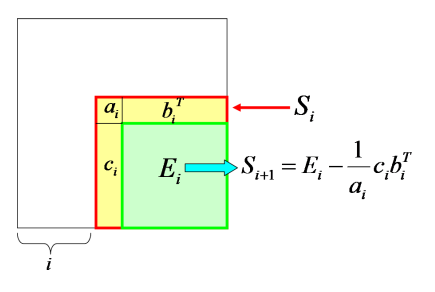
\includegraphics[width=80mm]{images/ldu_frac_algorithm.eps}
\caption{LDU Factorization Algorithm}
\end{center}
\end{figure}

\subsubsection{Compute Components}

Let's write the above algorithm for each component. As the original matrix $\bi{A}$, the components of the LDU decomposed matrix are as follows.
However, suppose that you write ij components of $A,L,D,U$ like $a_{ij}$ respectively.

\begin{eqnarray}
d_{ij} =
\left\{\begin{array}{ll}
a_{ii} - \sum_{k=0}^{i-1}l_{ik} u_{ki} d_{kk}\;\; & (i=j)\\
0 & (i\ne j)
\end{array}\right.\;\;\;\; (i=0,1,\ldots,n-1)
\end{eqnarray}


\begin{eqnarray}
l_{ij} =
\left\{\begin{array}{ll}
\left(a_{ij} - \sum_{k=0}^{j-1} l_{ik} u_{kj} d_{kk}\right)/d_{jj}\;\; &  (i>j)\\ 1 &(i=j)\\
0 & (i<j)\end{array}\right.\;\;\;\; (i,j=0,1,\ldots,n-1)
\end{eqnarray}


\begin{eqnarray}
u_{ij} = \left\{\begin{array}{ll}
\left(a_{ij} - \sum_{k=0}^{i-1} l_{ik} u_{kj} d_{kk}\right)/d_{ii}\;\; & (i<j)\\
1 & (i=j)\\ 0 & (i>j)\end{array}\right.\;\;\;\; (i,j=0,1,\ldots,n-1)
\end{eqnarray}


\subsection{LU disassembly}

And the lower triangular matrix and the upper triangular matrix. This is called LU factorization. When $\bi{A}$ is asymmetric, Craut's decomposition is called, in the case of symmetry it is called Cholesky decomposition.

\subsubsection{LU decomposition part 1 (decomposition with 1 diagonal of L)}

Let $\bi{A}=\bi{L}\bar{D}\bar{U}$ be the matrix decomposed using LDU decomposition in the previous section.

\begin{equation}
\bi{U} = \bar{D}\bar{U}
\end{equation}

Then, since $\bi{U}$ is an upper triangular matrix,

\begin{equation}
\bi{A} = \bi{L}\bi{U}
\end{equation}

Let's write the above algorithm for each component with reference to LDU decomposition. As the original matrix $\bi{A}=\bi{L}\bar{\bi{D}}\bar{\bi{U}}$, the components of the LDU decomposed matrix are as follows. The following relational expression obtained for each component from $\bi{U} = \bar{\bi{D}}\bar{\bi{U}}$
$\bar{d}_{ii} = u_{ii}$, $u_{ij} = \bar{u}_{ij}\bar{d}_{ij}$
Then, the following is obtained.

\begin{eqnarray}
l_{ij} = \left\{\begin{array}{ll}
\left(a_{ij} - \sum_{k=0}^{j-1} l_{ik} u_{kj}\right)/u_{jj}\;\; &  (i>j)\\
1 &(i=j)\\
0 & (i<j)
\end{array}\right.\;\;\;\; (i,j=0,1,\ldots,n-1)
\end{eqnarray}


\begin{eqnarray}
u_{ij} = \left\{\begin{array}{ll}
a_{ij} - \sum_{k=0}^{i-1} l_{ik} u_{kj}\;\; & (i\le j)\\
0 & (i>j)\end{array}\right.\;\;\;\; (i,j=0,1,\ldots,n-1)
\end{eqnarray}


\subsubsection{LU decomposition part 2 (decomposition with one diagonal of U)}

Let $\bi{A}=\bar{\bi{L}}\bar{D}\bi{U}$ be the matrix decomposed using LDU decomposition in the previous section.

\begin{equation}
\bi{L} = \bar{L}\bar{D}
\end{equation}

Then, since $\bi{U}$ is an upper triangular matrix,

\begin{equation}
\bi{A} = \bi{L}\bi{U}
\end{equation}

Let's write the above algorithm for each component with reference to LDU decomposition. As the original matrix $\bi{A}=\bar{\bi{L}}\bar{\bi{D}}\bi{U}$, the components of the LDU decomposed matrix are as follows. The following relational expression obtained for each component from $\bi{L} = \bar{\bi{L}}\bar{\bi{D}}$
$\bar{d}_{ii} = u_{ii}$, $u_{ij} = \bar{u}_{ij}\bar{d}_{ij}$
Then, the following is obtained.

\begin{eqnarray}
l_{ij} = \left\{\begin{array}{ll}
a_{ij} - \sum_{k=0}^{j-1} l_{ik} u_{kj}\;\; &  (i\ge j)\\
0 & (i<j)\end{array}\right.\;\;\;\; (i,j=0,1,\ldots,n-1)
\end{eqnarray}


\begin{eqnarray}
u_{ij} = \left\{\begin{array}{ll}
\left(a_{ij} - \sum_{k=0}^{i-1} l_{ik} u_{kj}\right)/l_{ii}\;\; & (i< j)\\
1 & (i=j) \\
0 & (i>j)\end{array}\right.\;\;\;\; (i,j=0,1,\ldots,n-1)
\end{eqnarray}

This is often used as a data structure of a matrix when CRS data format is used.

\subsection{Solving simultaneous linear equations}

Let's solve the simultaneous linear equation as follows.

\begin{equation}
\bi{A}\bi{x} = \bi{y}
\end{equation}

Here, if the coefficients are LU decomposed as follows,

\begin{equation}
\bi{A} = \bi{L}\bi{U}
\end{equation}

To solve this, we introduce the vector $\bi{z}$ as follows, first solve for the lower triangular matrix, then solve for the upper triangular matrix in order. When solving for the lower triangular matrix and the upper triangular matrix, solutions are obtained by forward substitution and backward substitution as described later.

\begin{equation}
\bi{z} = \bi{L}^{-1}\bi{y}
\end{equation}


\begin{equation}
\bi{x} = \bi{U}^{-1}\bi{z}
\end{equation}


\subsubsection{How to find z by solving Lz = y}

Can be done using forward substitution

\begin{eqnarray}
\bi{L}\bi{z} &=& \bi{y}\\
l_{00}z_0 &=& y_0\;\;\; \Leftrightarrow\;\;\; z_0 = y_0/l_{00}\\
l_{10}z_0 + l_{11}z_1 &=& y_1\;\;\; \Leftrightarrow\;\;\; z_1 = \{y_1-l_{10}z_0\}/l_{11}\\
l_{20}z_0 + l_{21}z_1 + l_{22}z_2 &=& y_2\;\;\; \Leftrightarrow\;\;\; z_2 = \{y_2-l_{20}z_0-l_{21}z_1\}/l_{22}\\
\sum_{i=0}^k l_{ki}z_i &=& y_k\;\;\; \Leftrightarrow\;\;\; z_k = \{y_k-\sum_{i=0}^{k-1}l_{ki}z_i\}/l_{kk}\;\;\;\;(k=0,1,\ldots,n-1)
\end{eqnarray}


\subsubsection{How to obtain x by solving Ux = z}

Can be obtained using backward elimination.

\begin{equation}
\bi{U}\bi{x} = \bi{z}
\end{equation}

From the last element of x, we will seek to the first element in order

\begin{eqnarray}
&&u_{(n-1,n-1)}x_{n-1} = z_{n-1}\nonumber\\
&&\;\;\;\Leftrightarrow \;\;\; x_{n-1} = z_{n-1}/u_{(n-1,n-1)}\\
&&u_{(n-2,n-2)}x_{n-2} + u_{(n-2,n-1)}x_{n-1} = z_{n-2}\nonumber\\
&&\;\;\;\Leftrightarrow \;\;\; x_{n-2} = \{z_{n-2}-u_{(n-2,n-1)}x_{n-1}\}/u_{(n-2,n-2)}\\
&&u_{(n-3,n-3)}x_{n-3} + u_{(n-3,n-2)}x_{n-2} + u_{(n-3,n-1)}x_{n-1} = z_{n-3}\nonumber\\
&&\;\;\;\Leftrightarrow \;\;\; x_{n-3} = \{z_{n-3}-u_{(n-3,n-1)}x_{n-1}-u_{(n-3,n-2)}x_{n-2}\}/u_{(n-3,n-3)}\\
&&\sum_{i=1}^k u_{(n-k,n-i)}x_{n-i} = z_{n-k}\nonumber\\
&&\;\;\;\Leftrightarrow \;\;\; x_{n-k} = \{\sum_{i=1}^k z_{n-k}-u_{(n-k,n-i)}x_{n-k}\}/u_{(n-k,n-k)}\;\;\;(k=1,2,\ldots,n)
\end{eqnarray}


\subsection{Speed ​​up compression display and calculation}

In addition to the original matrix $\bi{A}$ before decomposition it is inefficient to reserve separate memory to express L and U. L is a lower triangular matrix, the upper half is 0, U is the lower triangular matrix, and the lower half is 0. By transforming the original matrix so that the upper half is U and the lower half is L, you can display them in one matrix.
Let us now consider the case where LU factorization is performed so that the diagonal of U is 1. That is, $A=\left(\bar{L}\bar{D}\right)\bi{U} = LU$ transforms $\bi{A}$ at this time so that it becomes a matrix $\bi{A}'$ like the following. However, let izz components of $\bi{A}',\;\bi{L},\;\bi{U}$ be $a'_{ij}$, $l_{ij}$, $u_{ij}$ respectively.

\begin{eqnarray}
a'_{ij} = \left\{\begin{array}{ll}l_{ij} & (i>j)\\ 1/l_{ii} & (i=j) \\ u_{ij} & (i<j)\end{array}\right.
\end{eqnarray}

Notice that the diagonal elements of $A'$ are the inverse of the diagonal elements of $\bi{L}$. This is because the diagonal elements of $\bi{A}'$ are used for LU decomposition and diagonal elements for forward substitution, but they are always used as opposite values, so you can expect high speed by storing the opposite value. Now, LU decomposition such that the diagonal of U is 1 is suitable for line by line decomposition. This can be said to be the most suitable decomposition method for row-wise data structures like CRS. The algorithm for finding such a matrix $\bi{A}'$ is as follows.

\subsubsection{LU factorization (LU decomposition with U diagonal 1, compressed display with diagonal reciprocal)}

\begin {enumerate}
\item $for\;\; i=0,\ldots,n-1$
\begin {enumerate}
\item $for\;\; j=0,\ldots,n-1$
\begin {itemize}
\item $a'_{ij} = a_{ij} - \sum_{k=0}^{j-1} a'_{ik} a'_{kj}$
\end {itemize}
\item $end\; for$
\item $a'_{ii} = 1/ a'_{ii}$ (Calculate and store the reciprocal of diagonal elements of lower triangular matrix)
\item $for\;\; j=i+1,\ldots,n-1$
\begin {itemize}
\item $a'_{ij} = a'_{ij}\times a'_{ii}$ (Multiply diagonal elements of lower triangular matrix to create upper triangular matrix)
\end {itemize}
\item $end\; for$
\end {enumerate}
\item $end\; for$
\end {enumerate}

Now, the forward elimination and the backward substitution for the deformed matrix are as follows.

\subsubsection{Forward substitution (LU decomposition with U diagonal 1, compressed display with diagonal reciprocal)}


\begin{equation}
z_k = \{y_k-\sum_{i=0}^{k-1}a'_{ki}z_i\}a'_{kk}\;\;\;\;(k=0,1,\ldots,n-1)
\end{equation}


\subsubsection{Back substitution (LU decomposition with U diagonal 1, compressed display with diagonal reciprocal)}


\begin{equation}
x_{n-k} = \sum_{i=1}^k z_{n-k}-a'_{(n-k,n-i)}x_{n-i}\;\;\;(k=1,2,\ldots,n)
\end{equation}


\subsubsection{LU decomposition algorithm diagram (compressed display)}

FIG. 2 shows an LU decomposition algorithm when compressed display is performed. It does not depend on the type of LU decomposition or the decomposition procedure, and it is roughly as shown in the following figure. In other words, if there is an element $a_{ij}$ to decompose, refer to all the elements of \ textbf {decomposed} of $a_{kj}$ and left $a_{ik}$ so that the diagonal elements $a_{kk}$ and $a_{ij}$ can make a rectangle.

\begin{figure}
\begin{center}
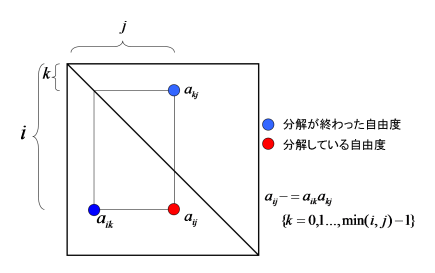
\includegraphics[width=80mm]{images/decomp_matrix.eps}
\caption{illustragtion of LU factorization where L and U are put in the same matrix.}
\end{center}
\end{figure}



\end{document}
